%%% Notice: This file contains a large number of \verb's 
%%%         or verbatim environments in order to display command names
%%%         or examples.  But the use of \verb/verbatim is *not* recommended. 
%%% ver.7 2018/05/15 
\documentclass{pasj02}
%\draft 
\Received{$\langle$reception date$\rangle$}
\Accepted{$\langle$acception date$\rangle$}
\Published{$\langle$publication date$\rangle$}
%% \SetRunningHead{Astronomical Society of Japan}{Usage of \texttt{pasj00.cls}}
%% \SetRunningHead{Astronomical Society of Japan}{Usage of \texttt{pasj00.cls}}


\begin{document}

\title{The Impact of Relativistic Effects on the Analysis of Magnetar Hot Spots}
\author{Chushu \textsc{Qu}\altaffilmark{1}}%
\email{sojo@g.ecc.u-tokyo.ac.jp}

\author{Yudai \textsc{Suwa}\altaffilmark{1,2}}%

\author{Teruaki \textsc{Enoto}\altaffilmark{3}}%

% \author{friends}

\altaffiltext{1}{Department of Earth Science and Astronomy, The University of Tokyo, Tokyo 153-8902, Japan}
\altaffiltext{2}{Center for Gravitational Physics and Quantum Information, Yukawa Institute for Theoretical Physics, Kyoto University, Kyoto 606-8502, Japan}
\altaffiltext{3}{Department of Physics, Kyoto University, Kyoto 606-8502, Japan}


\KeyWords{magnetar${}_1$ --- light bending${}_2$ --- NICER${}_3$ --- XMM-Newton${}_4$}

\maketitle

\begin{abstract}
Magnetars, known for their intense magnetic fields, emit soft X-ray emissions ($\le$10 keV) believed to originate from hot spots on their surfaces. In regions where a potent dipole magnetic field traverses from the inner to the outer star, there is a consequential plastic flow, resulting in an internal energy release. This phenomenon is responsible for heating the surface and creating the observed hot spots. In our study, we constructed a hot spot model, factoring in gravitational relativistic effects, to analyze the magnetar's pulse profile. By considering light-bending effect, we managed to reproduce the magnetar's (SGR 1833-0832, 1E 1048.1-5937 and 1E 1547.0-5937) pulse profile using our single hot spot model, offering a potential constraint on the strength and structure of the magnetic field.
\end{abstract}

\section{Introduction}


\section{Hot spot model}

\indent Since soft X-ray emission from a magnetar primarily originates from a hot spot on its surface. We developed the hot spot model to reproduce light curves from several parameters. The basic picture of this model which shows in Figure 1 includes a circular region on the sphere's surface represents the hot spot, with its size denoted by the angle $\rho$.

% \setcounter{figure}{0}
\begin{figure}[hbtp]
 \centering
 \includegraphics[keepaspectratio, scale=0.3]
      {hotspot.eps}
 \caption{View of a magnetar with one emitting hot spot on the surface. The angle between the rotation axis and center of hot spot is shown with $\theta$ and the angle between the rotation axis and observer is shown with $i$. While $\rho$ represents the size of the hot spot.}
 \label{}
\end{figure}

When the magnetar rotates in angular velocity $\Omega$, hot spot and its emission flux observed will alter simultaneously. If we define $\vec{O}$ as the unit vector towards observer and $\vec{n}$ as the spot normal, we could calculate the inclination by $\mu = \vec{O}\cdot\vec{n}$. Assume that the size of hot spot is small enough compare to magnetar radius R, which means hot spot is the point source, $\mu$ will change with time $t$ like (1)

\begin{equation} \label{2.1}
\mu(t)=\sin\theta\sin i\cos\Omega t+\cos\theta\cos i.
\end{equation}

\begin{table}[hbtp]
  \caption{Summary of the Parameters for Magnetars}
  \label{table:data_type}
  \centering
  \begin{tabular}{lr}
    \hline \hline
    Basic parameter & Symbol \\
    \hline \hline
    Period & \( P \) \\
    Period derivative & \( \dot{P} \) \\
    Magnetar Mass & \( M\) \\
    Magnetar Radius & \( R \) \\
    Distance & \( D \) \\
    Angular velocity & \( \Omega \) \\
    Viewing angle & \( i \) \\
    Colatitude of hot spot & \( \theta \) \\
    Phase of hot spot & \( \phi \) \\
    Size of hot spot & \( \rho, z \) \\
    Normalization flux & \( m \) \\
    \hline
  \end{tabular}
\end{table}

% \subsection{Light bending effect}

% \indent Magnetars, distinguished by their intense magnetization, are neutron stars with a density high enough to significantly bend light. A magnetar's compactness is defined by its mass, $M$, and represented through the Schwarzschild radius, $r_g=2GM/c^2$ where $G$ is the gravitational constant and $c$ is the speed of light.  For a typical neutron star with a mass of about 1.4 $M_{\odot}$ and a radius of approximately 12 km, the compactness ratio $r_g/R$ is roughly $\frac{1}{3}$. This ratio has been adopted as a fixed value in our analysis. For $R\ge 2r_g$, Beloborodov \citep{beloborodov2002gravitational} gave a high accuracy simple formula to quantify this relativistic effect. 

% Consider emission point is located at point $E$ at a radius $R$ (Figure 2.2). A photon emitted at some angle measured by the local observer $\alpha$ with respect to radius escapes along a bent trajectory. Now if we choose Schwarzschild coordinates $x^k=(t,r,\theta,\psi)$, the metric is given by

% \begin{equation} \label{2.2}
% ds^2=-(1-\frac{r_g}{r})dt^2+(1-\frac{r_g}{r})^{-1}dr^2+r^2d\theta^2+r^2\sin^2\theta d\psi^2
% \end{equation}

% We could find that the trajectory is in the plane $\theta=\ang{90}$. Assume $u^k = dx^k/d\lambda$ as the 4-velocity of the photon ($ds^2=0$), the integrals of the trajectory along $t$ and $\psi$ is $u^t=1$ and $u_{\psi}=b$. From $u^iu_i=0$ one finds $(u^r)^2=1-(b^2/r^2)(1-r_g/r)$. Noted that $\psi=0$ is the escape direction, we have

% \begin{equation}
% \psi=\int_R^{\infty}\frac{dr}{r^2}[\frac{1}{b^2}-\frac{1}{r^2}(1-\frac{r_g}{r})]^{-1/2}.
% \end{equation}


% \noindent The emission angle $\alpha$ has $\tan\alpha =\sqrt{u^{\psi}u_{\psi}}/\sqrt{u^ru_r}$ which yields

% \begin{equation}
% \sin\alpha=\frac{b}{R}\sqrt{1-\frac{r_g}{R}}
% \end{equation}

% \noindent Combining equations (2.2) and (2.3) one can compute numerically the relation between $\psi$ and $\alpha$ for a given $R$. At small $\eta=r_g/R$ one can expand equation (2.3) in $t$ and keep the liner term only. Using the equality $\int_0^{\sin\alpha}(\sin\alpha-z^3)(1-z^2)^{-3/2}dz=2(1-\cos\alpha)$ one gets $\psi=\alpha+\eta(1-\cos\alpha)/\sin\alpha+O(\eta^2)$.

% Beloborodov \citep{beloborodov2002gravitational} give a fantastic approximate relation of $\alpha$ and $\psi$

% \begin{equation}
% 1-\cos\alpha=(1-\cos\psi)(1-\frac{r_g}{R})
% \end{equation}

% \begin{figure}[hbtp]
%  \centering
%  \includegraphics[keepaspectratio, scale=0.2]
%       {photon_trajectory.eps}
%  \caption{Illustration of photon trajectory.}
%  \label{}
% \end{figure}

% Consider a star with a radius $R$, emitting radiation of varying intensity $I_0(\alpha)$ over its surface. An observer is located far away from the star, at a position represented by a radius vector $\vec{D}$, where $\vec{D} \gg R$. The observable surface element of the star, denoted as $dS = R^2d\mu d\varphi$, is characterized by $\mu = \cos\psi$ and $\varphi$ (an azimuthal angle relative to $\vec{D}$). The radiation flux $dF$ observed from this element depends on its projected area on the observer's sky, which can be expressed as a solid angle $d\omega = bdbd\varphi/D^2$. Here, $b$, the impact parameter, is a function of $\mu$ alone and represents the perpendicular distance from the line of sight to the observer. The flux $dF$, observable from the element $dS$, is then $dF=Id\omega$, where $I$ is the observed intensity. Due to gravitational redshift effects near the star, $I$ is reduced from the emitted intensity $I_0$, factored by $(1-\frac{r_g}{R})^2$, where $r_g$ is the Schwarzschild radius. Thus, $I = (1-\frac{r_g}{R})^2I_0$. Applying equation (2.3), we can calculate the observed radiation flux from the star's surface as

% \begin{equation}
% dF=\frac{Ib}{R}\frac{db}{d\mu}\frac{dS}{D^2}=(1-\frac{r_g}{R})I_0(\alpha)\cos\alpha\frac{d\cos\alpha}{d\mu}\frac{dS}{D^2}.
% \end{equation}

% \noindent Now applying the approximate relation (2.4) into (2.5), we get

% \begin{equation}
% dF=(1-\frac{r_g}{R})^2I_0(\alpha)\cos\alpha\frac{dS}{D^2}.
% \end{equation}

% \noindent It is recognized that emission from hot spot is the blackbody radiation, therefore the emission intensity should be a constant. Giving the normalized flux parameter $m=(1-r_g/R)^2I_0s/D^2$ ($s$ is the spot area), we could get

% \begin{equation}
% dF=m[\mu(i,\theta,\phi,t)(1-\frac{r_g}{R})+\frac{r_g}{R}].
% \end{equation}

% \noindent Besides Beloborodov's work, other researchers have also conducted significant studies on X-ray emission from rotating neutron stars \citep{bogdanov2019constraining,shapiro2008black}. These studies underscore that both compactness and rotation are critical in shaping emissions. A key development in this area is the Schwarzschild + Doppler approximation, which is particularly applied for uniformly rotating neutron stars (rotation frequency \textless 100 Hz). This approximation is expressed as follows:

% \begin{equation}
% v = \Omega R(1-r_g/R)^{-1/2}\sin\theta,
% \end{equation}

% \begin{equation}
% \delta = \frac{1}{\gamma[1-(v/c)\cos i]},
% \end{equation}

% \begin{equation}
% dF=(1-\frac{r_g}{R})^2[\frac{r_g}{R}+(1-\frac{r_g}{R})\mu]\delta^5I^{\prime}(\alpha)\frac{dS^{\prime}}{D^2}
% \end{equation}

% \noindent where $\gamma=[1-(v/c)^2]^{-1/2}$ is the Lorentz factor, and $\xi$ is the angle between the photon's propagation direction and the rotation axis. In terms of magnetars, the velocity $v$ is relatively small because $\Omega R\sim10^6\,\text{cm/s}(\frac{\Omega}{2\pi0.2\,\text{Hz}})(\frac{R}{10\,\text{km}})$, hence $\frac{v}{c}$ is a negligible value. As a result, $\delta$ approximates to 1. Consequently, equations (2.11) can be simplified to the form of equation (2.7).

% \noindent In this simplified model, proper time in the Schwarzschild metric is expressed as $d\tau^2=(1-\frac{r_g}{R})dt^2$, implying a direct relationship between the observed and emitted energies as shown in equation (2.12)

% \begin{equation}
% E=(1-\frac{r_g}{R})^{1/2}E^{\prime}.
% \end{equation}

Magnetars, as the special category of neutron stars, hold mass about 1.4 solar mass and radius in the order of 10 kilometers. Therefore, we could never ignore the effect of general relativity when considering emission come from its surface. In this study, we introduced Beloborodov 2002 to give a reasonable approximation about light bending effect, which showed in Figure 2.

\begin{figure}[hbtp]
 \centering
 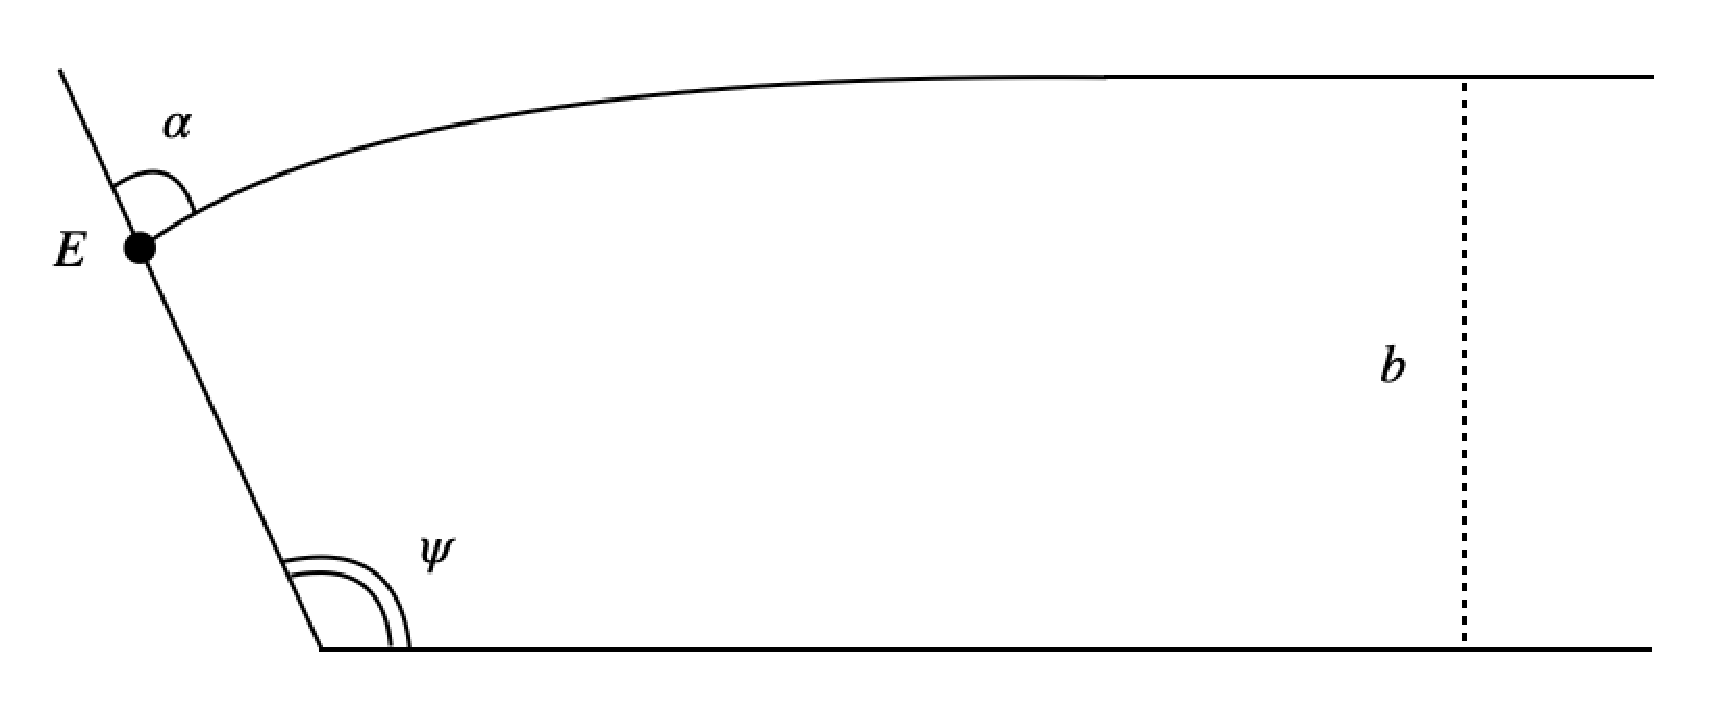
\includegraphics[keepaspectratio, scale=0.2]
      {photon_trajectory.eps}
 \caption{Illustration of photon trajectory under strong gravity field. Point $E$ stands for initial photon position. $alpha$ represents local direction of photon's path and $\psi$ shows the final direction. Beloborodov 2002 gave relation to $\alpha$ and $\psi$ by $1-\cos\alpha=(1-\cos\psi)(1-\frac{r_g}{R})$.}
 \label{}
\end{figure}

Giving the normalized flux parameter $m$, we could get

\begin{equation}
dF=m[\mu(i,\theta,\phi,t)(1-\frac{r_g}{R})+\frac{r_g}{R}].
\end{equation}

% \subsection{Method to reproduce emission size}

% \indent In our study, we adopt a method to simulate the distribution of hotspots on a magnetar's surface (Leopardi 2007). This method could uniformly arrange point sources within a circular region, mimicking the emission size of the hot spot on the magnetars.

In our study, we adopt a method to simulate the distribution of hot spots on a magnetar's surface (Leopardi 2007). This method could uniformly arrange point sources within a circular region, mimicking the emission size of the hot spot on the magnetar.

The technique begins with the linear distribution of z-coordinates for each point source. These coordinates are evenly spaced between $z_0R$ and $R$, where $R$ is the sphere's radius and $z_0$ is the fraction that doesn't arrange any points. This linear spacing is key to mapping out the vertical extent of the circular region in three-dimensional space.

Crucially, the method employs the golden ratio, $\frac{1+\sqrt{5}}{2}$, for the angular distribution of points around the sphere. This approach ensures a uniform spread of points, effectively avoiding clustering. We arrange $\theta$ and $\phi$ of i th points as (3)-(5),

\begin{equation}
    i^{\prime} = i-0.5,
\end{equation}

\begin{equation}
    z = 1-i^{\prime}(\frac{1-z_0}{N}),
\end{equation}

\begin{equation}
    \theta_{i^{\prime}} = \frac{4\pi i^{\prime}}{1+\sqrt{5}}.
\end{equation}


$N$ is the total number of point sources  and the specified emission region in z-coordinates $(1-z_0)R$, we are able to closely replicate the hotspots on the magnetar's surface, as demonstrated in Figure 3. 

\begin{figure}[hbtp]
 \centering
 \includegraphics[keepaspectratio, scale=0.35]
      {golden_ratio.eps}
 \caption{A series of golden ratio arrangement for different $\rho$}
 \label{}
\end{figure}

% \section{Timing analysis}

% Supposing point source emission ($s\rightarrow0$), we have

% \begin{equation} \label{eq6}
% dF(t)=m[\sin\theta\sin i\cos\Omega t+\cos\theta\cos i(1-\frac{r_g}{R})+\frac{r_g}{R}]
% \end{equation}

% \subsection{Relativistic correction for spectrum analysis}

In this study, we employed the X-ray spectral fitting program Xspec, a key component of the High Energy Astrophysics Software (HEASoft) package, to extract information about the emission size. Xspec includes the 'bbodyrad' model, which is instrumental in deriving emission area and temperature from spectral data. This facilitates a comprehensive comparison of hot spot size obtained from both timing and spectral analysis. Given that X-ray emissions undergo absorption while propagating through the interstellar medium, we utilized the 'tbabs' model (Wilms et al. 2000) to estimate this effect. In our analysis, the combination of 'tbabs' and 'bbodyrad' models was applied to fit the spectrum. The fitting equation of 'bbodyrad' showed in (6), 

% To lay the groundwork for our fitting procedure, we first consider the equation for a blackbody

% \begin{equation} \label{eq14}
% B_{\nu}=\frac{2h\nu^3}{c^2}\frac{1}{\exp(\frac{h\nu}{kT})-1}
% \end{equation}

% Since we are modelling radiation from the star, therefore

% \begin{equation} \label{eq15}
% F_{\nu} = \int I\cos\theta d\Omega = B_{\nu}\int_{0}^{2\pi}d\phi\int_{0}^{\theta_c}\sin\theta\cos\theta d\theta
% \end{equation}

% $\theta_c = \arcsin{R/D}$, this gives

% \begin{equation} \label{eq16}
% F_\nu = \pi B_\nu (\frac{R}{D})^2
% \end{equation}

% Since $E=h\nu$ we could get $F_E$

% \begin{equation} \label{eq16}
% F_EdE = \frac{2\pi E^2}{h^3c^2}\frac{1}{\exp(E/kT)-1}(\frac{R}{D})^2dE
% \end{equation}

% 'bbodyrad' replace $(\frac{R}{D})^2$ with normalization factor K in unit of $(\frac{R_{km}}{D_{10kpc}})^2$. Finally, we could give

\begin{equation}
A(E) = \frac{K\times 1.0344\times 10^{-3}E^2dE}{\exp(E/kT)-1}
\end{equation}

We could extract emission radius from the spectrum analysis, however, 'tbabs*\\bbodyrad' didn't account for any relativistic effect. If we consider light bending effect in (6) as well as temperature correction cause by Doppler shift, we get $A^\prime(E^\prime)=A(E)/(1-\frac{r_g}{R})^2$, $E^\prime=E/(1-\frac{r_g}{R})^{1/2}$, that is

\begin{equation}
K^\prime = K(1-\frac{r_g}{R})^{-1/2}.
\end{equation}

So would the emission radius after relativistic correction be

\begin{equation}
R^\prime_{spec} = R_{spec}(1-\frac{r_g}{R})^{-1/4}.
\end{equation}

% \section{Parameter estimation}

% We performed Markov Chain Monte Carlo (MCMC) method to determine the best parameter set $X$ that has best fit with the pulse profile. $X$ is defined by

% \begin{equation} \label{eq8}
% X = \lbrace i,\theta,\phi,\rho, m\rbrace
% \end{equation}

% instruction of emcee

% \subsection{Data analysis}

% In order to investigate soft X-Ray emission of hot spots, we chose to analyse NICER events in the energy range of 1-5 keV. We downloaded archive data from HEASARC Archive (\url{https://heasarc.gsfc.nasa.gov/docs/archive.html}). Before downloading archive data, we first screen magnetars suitable for conducting this research taking advantage of McGill Online Magnetar Catalog (\url{https://www.physics.mcgill.ca/~pulsar/magnetar/main.html}). The data were processed using HEASOFT version 6.32.1 and NICERDAS version 11a. The calibration was done by taking advantage of CALDB release for NICER observation. 

% The energy band of both timing data and spectrum data were fixed from 1 keV to 5 keV. By setting the same energy band filter, we could compare the same physics parameters extracted from both timing and spectrum analysis. In addition, we applied a average count rate filter for each magnetar in light curve to select the data when magnetars were in quiescent emission state.

% Figure 2.10 shows the long time light curve of 1E1048.1-5937 for instance , each point stands for a single epoch of observation (usually last from handreds seconds to thousands seconds). We choose the data that has the longest exposure while average count rates is low, too. The data we use is listed in Table 3.1.

% \begin{figure}[hbtp]
%  \centering
%  \includegraphics[keepaspectratio, scale=0.27]
%       {long_time_lc.eps}
%  \caption{}
%  \label{long_lc}
% \end{figure}

% The NICER data comprises four processing levels. Level 0 is the raw data received by NICER, which is typically packaged into small segments to facilitate data communication between the spacecraft and ground stations. The NICER science data pipeline system is responsible for reassembling these segments into Level 1 data. Consequently, data sets in the HEASARC do not include Level 0 data. Level 1 data are organized in chronological order and are free of duplicated information. With 52 detectors in total, NICER uses 7 Measurement and Power Units (MPUs) for data readout. As a result, NICER's data always include unfiltered data files, named as 'ni\{ObsID\}\_0mpu\{MPU Number\}\_ufa.evt'. Whenever data are downloaded from HEASARC, they are provided as Level 1 data. 

% The 'nicerl2' task, a component of the HEASoft software package, is employed to calibrate and screen Level 1 data. The output of this process are files named 'ni\{ObsID\}\_0mpu\{MPU Number\}\_cl.evt' and 'ni\{ObsID\}.mkf,' where 'cl' stands for 'clean,' and 'mkf' represents 'make filter.' Subsequent to this process, data analysis is bifurcated into two threads: one for timing construction and the other for spectral analysis. We will first discuss the timing analysis thread.

% We use xselect to extract the light curve, applying the 'filter pha\_cutoff 100 500' command to specifically filter the photon energy range, effectively eliminating data below 1 keV and above 5 keV.  

% After obtaining the Level 3 light curve data, the 'barycorr' tool is applied to correct the arrival times of X-ray photons to the solar system's barycenter. This vital correction accounts for the Earth's motion, ensuring accurate timing of the observed phenomena and consistency with observations from other telescopes across different time periods. In our study, the JPL Ephemeris DE430 (JPLEPH430) was utilized for these barycentric corrections.

% % add precise input info

% Then we used 'powspec', a tool designed to generate power density spectra, to facilitate the identification of periodicities within the X-ray data. The newbin time is settled to 5e-5 s while number of newbin inputed as 2e6 to cover the single period of pulse in the light curve. Following this, 'efsearch' was deployed to conduct an epoch-folding search. This technique is instrumental in refining the periodicities initially identified by 'powspec', through an iterative process of data folding across an array of trial periods, thereby ascertaining the most precise periodic signal. The initial input of period was inputted based on McGill Online Magnetar Catalog. The culmination of this analytical sequence conducted by 'efold', which is utilized to construct pulse profiles based on the accurately determined periods. Phasebins of all data is 32 to give a good resolution to both phase and count rates.

% In our spectral analysis, we employed 'nibackgen3C50', 'nicerarf', and 'nicerrmf' for the generation of background files, Ancillary Response Files (ARFs), and Response Matrix Files (RMFs), respectively.

% The 'nibackgen3C50' tool utilizes an empirical background model for NICER spectral analysis \citep{Remillard_2022}. This model innovatively leverages various background proxies present in NICER data to establish the foundational states of the background database. Key among these proxies are the graded event data, which differentiate X-ray events based on their interaction points within each detector. Specifically, the model discerns between events occurring near the center of each detector and those near the detector edge under a field aperture.

% The 'nicerrmf' tool incorporates several effects that influence the detector's resolution and charge collection efficiency. Considering that detectors 14 and 34 exhibit significant noise in their output, we have excluded data from these detectors in our analysis. Modeling, calibration data and optical loading act as key components in this task. 

% Similarly, task 'nicerarf' works for characterizing the transmission properties of the NICER X-ray Concentrators, the transmission throughput of filters and windows, and the detector quantum efficiency. The RA and Dec we used for inputs in both nicerarf and nicerrmf is adapted from HEASARC coordinate converter (\url{https://heasarc.gsfc.nasa.gov/cgi-bin/Tools/convcoord/convcoord.pl}).

\section{Mock Simulation}
We conduct mock simulations to investigate the relationship between the spectral radius and the radius of the pulse model. The spectral radius is derived from the time-integrated energy flux during rotational phases (bolometric spectra), while the model radius corresponds to the static geometry of the system without accounting for time-averaged effects. Due to relativistic effects, analytical corrections are challenging to implement, making mock simulations a practical approach to uncover the relationship between these two radii.

By simulating the observed flux as a function of rotational phase and integrating it over time, we aim to quantify the transformation required to compare the spectral radius with the model radius directly.

Since the relativistic constant has been fixed to $\frac{1}{3}$, we only need to consider parameters that are the viewing angle $i$ and the angle between the hot spot and the rotation axis$\theta$. Thus, a pair of $i$ and $\theta$ would be roughly limited.

\section{Result}

The red clump star method was used to measure the distances of 1E 1048.1-5937 and XTE J1810-1907. Utilizing data from the 2MASS catalog, this method involves constructing color-magnitude diagrams (CMDs) from nearby stars, identifying the distribution of red clump stars, and fitting a Gaussian function to ascertain the peak. The method then calculates reddening and distance by translating the J-K versus K data, taking advantage of the known properties of red clump stars. For 1E 1547.0-5408, a different approach, the dust scattering method, was employed. This technique measures distances by analyzing X-ray scattering from interstellar dust grains. When a cosmic source emits an X-ray burst, the radiation scatters off dust layers, forming observable, expanding rings. The angular size of these rings increases over time, allowing for the determination of both the dust layer's and the X-ray source's distances through analysis of the ring's expansion rate and intensity decay.

\subsection{1E 1048.1-5937}
!!!!!ObsID 1020240106のデータを使っているがNICER
には他にもっと長いexposureを持つ非outburst期間のデータがある。--250110

使用したデータに対しての説明も必要?

1E 1048.1-5937, a persistent X-ray source, was first discovered by the Einstein X-ray Observatory (Steward et al. 1986). NICER began observing this magnetar in 2007, contributing dozens of observational datasets, each with exposure times exceeding 2000 seconds. Recognized as one of the most active magnetars, 1E 1048.1-5937 has undergone several outbursts over the years (Tam et al. 2007; Archibald et al. 2014, 2020). Notably, this magnetar emits radio radiation exclusively during its outburst phases, while at other times, it is limited to X-ray and optical emission.
In our analysis, we utilized data from ObsID 1020240106, which recorded an average count rate of 4.04 counts per second (with a binning factor of 16) over an exposure time of 4365.48 seconds. These observations confirm the magnetar's periodicity at approximately 6.4632 seconds, with a period derivative of $2.24\times10^-11$. 

\begin{figure}[htbp]
\begin{center}
\includegraphics[width=.9\linewidth]{1E1048newtonian.eps}
\caption{}\label{fig:1E1048newton}
\end{center}
\end{figure}

\subsection{1E 1547.0-5408}
1E 1547.0-5408 was first detected in 1980 by the Einstein X-ray satellite, but it was identified as a magnetar in 2007 \citep{gelfand2007compact}. In our analysis, we used data from ObsID 2515010201, which recorded an average count rate of 1.86 counts per second (with a binning factor of 16) over an exposure time of 3651 seconds. The observed period of this magnetar is 2.07 seconds, with a period derivative of $4.79\times10^{-11}$. Figure 3.6 presents the power spectrum and the peak search results for 1E 1547.0-5408. The power spectrum reveals a peak near 0.5 Hz, and the period searching analysis for this peak indicates the best $\chi^2$ fit at 2.0886 seconds.


\subsection{XTE J1810-197}
XTE J1810-197 was first detected in 2003 \citep{ibrahim2004discovery}. In our analysis, we used data from ObsID 3661010306, which recorded an average count rate of 5.87 counts per second (with a binning factor of 16) over an exposure time of 18839 seconds. The observed period of this magnetar is 5.54 seconds, with a period derivative of $7.76\times10^{-12}$. Figure 3.11 presents the power spectrum and the peak search results for XTE J1810-197. The power spectrum reveals a peak slightly lower than 0.2 Hz, and the period search analysis for this peak indicates the best fit $\chi^2$ at 5.542 seconds.


\subsection{Swift J1555.2-5402}
Swift J1555.2-5402 was first detected in 2021 \citep{enoto2021month}. In our analysis, we used data from ObsID 4560010102, which recorded an average count rate of 4.15 counts per second (with time bins of 30 s) over an exposure time of 18839 seconds. The observed period of this magnetar is 3.86 seconds, with a period derivative of $3.05\times10^{-11}$. Figure 3.16 presents the power spectrum and the peak searching results for Swift J1555.2-5402. The power spectrum reveals a peak about 0.25 Hz, and the period searching analysis for this peak indicates the best $\chi^2$ fit at 3.8609 seconds.


\section{Summary}
We apply timing and spectrum analyze while compare the result of these two to lead out the consistency between their results.

\section{Discussion}


\end{document}

